\documentclass[12pt,a4paper,danish,oneside,openany]{memoir} 
% Skabelon af DTU's LaTeX support gruppe, v20090423

\usepackage[utf8]{inputenc} 
%\usepackage{usecases}
\usepackage{vhistory}
\usepackage[danish]{babel} % danske overskrifter
\usepackage[T1]{fontenc}   % fonte (output)
\usepackage{lmodern}       % vektor fonte
\usepackage{graphicx}      % indsættelse af billeder
\graphicspath{ {./Figurer/} }
\usepackage{pdfpages}      % pdf som forside evt
\usepackage{morefloats}    % flere floats til tabeller
\usepackage{array}         % udvidet tabel 
\usepackage{listings}      % kode
% \usepackage{palatino}      % lækker font
% \linespread{1.3}           % kræver lidt mere line spacing
\usepackage{rotating}
\usepackage{tikz}

\addto\captionsdanish{
  \renewcommand{\contentsname}%
    {Indholdsfortegnelse}     %
} % Så bruger vi bare 'Indholdsfortegnelse' i stedet for 'Indhold'

\usepackage{underscore}
\usepackage{a4wide}
\usepackage{mathtools} % matematik - underst¿tter muligheden for at bruge \eqref{}

\usepackage[plainpages=false,pdfpagelabels,pageanchor=false]{hyperref} % aktive links

\usepackage{memhfixc}  % rettelser til hyperref

\usepackage{tipa}
\pretolerance=2500     % højt tal, mindre orddeling og mere space mellem ord.
% 3000 er okey, 1000 er for lidt, 5000 i overkanten, 8000 er for meget..

\usepackage[font=small,labelfont=bf,labelsep=endash]{caption}
 
\pagestyle{headings}

\makechapterstyle{mortenovi}{%
\setlength{\beforechapskip}{0cm}%længde fra top af side til kapitel-overskrifter
\setlength{\afterchapskip}{1cm}%længde fra kapiteltekst til body-tekst
\setlength{\midchapskip}{2cm}%længe mellem kapitelnummer og kapiteltekst
\renewcommand\chapnamefont{\normalfont\Large\scshape\raggedleft}
\renewcommand\chaptitlefont{\normalfont\Huge\bfseries\sffamily}
\renewcommand\chapternamenum{}%default "kapitel"
\renewcommand\printchapternum{%
    \makebox[0pt][l]{%
    \hspace{0.4em}
    \resizebox{!}{4ex}{\chapnamefont\bfseries\sffamily\thechapter}}
    }%"kapitel. x"-linjen og dens boxe og bredder - prøv at sætte xyz ind først på de tre linjer respektivt.
\renewcommand\afterchapternum{\par\hspace{1.5cm}\hrule\vspace{0.5cm}}
\renewcommand\afterchaptertitle{\vskip\onelineskip \hrule\vskip\afterchapskip
}}
\chapterstyle{mortenovi}

\maxtocdepth{subsection} %Only parts, chapters and sections in the table of contents
\settocdepth{subsection}

% \includeonly{forord,testing} % Kompiler kun de kapitler du arbejder med.

\topmargin = 0pt
\usepackage[textwidth = 155mm]{geometry}
\usepackage{tabularx}
\usepackage{booktabs} % http://ctan.org/pkg/booktabs 
\newcommand{\tabitem}{~~\llap{\textbullet}~~}

\begin{document}

\part*{System Design Document}


\chapter*{Introduction}

\section*{Design goals}

\paragraph{Usability: } The Calendar system should be designed with the goal in mind that it should be fairly easy to use by the Client. 

\paragraph{Response time: } The Calendar system should be quite responsive to user input, and commonly make actions in a matter of milliseconds. 

\paragraph{Extensibility: } The Calendar system should support the opportunity to extend the program and make it interact with different calendar programs such as Google Calendar, Exchange and iCal. 



%\section*{Overview}


\chapter*{Proposed system}

\section*{Overview}

\textbf{Architectural style}
\newline
 We decided to use the MVC pattern as the basic architectural style for the Calendar system.
\newline
\newline
The MVC pattern separates data and user interface and has Controller as a intermediated component. The pattern is used when there are multiple ways to view and interact with data.
\newline
\newline
MVC is a abbreviation for Model View Controller. The software is divided in these components. The components are defined as following:
\begin{itemize}
	\item \textbf{Model} handles data.
	\item \textbf{View} is attached to model and presents the data.
	\item \textbf{Controller} is the link between model and view. 
\end{itemize}
\bigskip


To get an overview of the MVC pattern we outlined the pros and cons.
\newline
\textbf{Pros}
\begin{itemize}
	\item low coupling
	\item high cohesion
	\item code maintenance
	\item code reuse
\end{itemize}
\textbf{Cons}
\begin{itemize}
	\item code complexity
	\item development time
\end{itemize}

\newpage
In our Object Oriented Analysis an Analysis Object Model was defined where we identified:
\begin{itemize}
	\item Entity objects (\emph{model})
	\item Boundary objebts (\emph{view})
	\item Control objects (\emph{controller})
\end{itemize}


The Analysis Object Model is a simplification of MVC pattern. It made it eaiser to set up the MVC pattern and build further on the Object Oriented Design. 

\newpage
\section*{Subsystem decomposition}
The subsystem CalendarManagement is the system where most of the program is placed. This system is responsible for all the local events happening in the system. This means that it would handle creation of the calendar, events and provide the necessary GUI for the local program. 

This subsystem has two connections outside the subsystem itself. The first one goes to "ShareInterface" that has all the necessary functions that the CalendarManagement system could ask for when it is about to share a calendar or an event. The other outgoing connection is to the SyncInterface. This is an interface that holds all the needed method calls to synchronize the calendar. Behind the two interfaces we have the subsystems ShareManagement and SyncManagement. 
\newline
\newline
The Share Management has to do with sending the information to the right people and using the right systems. The reason why we made this an interface is that it has been a commonly thing to share through facebook and other social media platforms. Therefore it would be nice to easily have the opportunity to extend the share option so that it would support e.g. Facebook. 
\newline
\newline
The subsystem SyncManagement is where we keep our calendars up to date, where we got the information, of whom the calendar belongs to, and which users that are invited to see it. The syncManagement keep the client calendars synchronized and handles the updates between the local calendar and the online ones. This is also behind an interface so that we can easily exchange it. That would turn to our advantage so the maintenance and upgrades of the system could be done easy. You simply exchange the subsystem part with a new one. E.g. if we wanted to update our synchronization part with a newer version of a data base program, the syncManagement is exchanged, but the rest could stay intact. 
\newline
\begin{figure}[ht!]
\centering
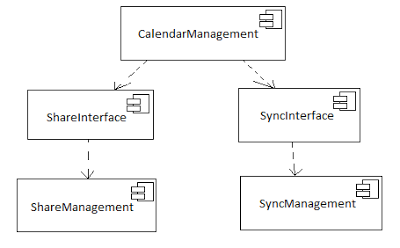
\includegraphics[width=90mm]{diagram.png}
\end{figure}

\end{document}